% Created 2018-02-11 Sun 17:54
\documentclass{article}
\usepackage[mathletters]{ucs}
\usepackage[utf8x]{inputenc}
\usepackage[T1]{fontenc}
\usepackage{fixltx2e}
\usepackage{graphicx}
\usepackage{longtable}
\usepackage{float}
\usepackage{wrapfig}
\usepackage{rotating}
\usepackage[normalem]{ulem}
\usepackage{amsmath}
\usepackage{textcomp}
\usepackage{marvosym}
\usepackage{wasysym}
\usepackage{amssymb}
\usepackage{hyperref}
\tolerance=1000
\usepackage[margin=1.0in]{geometry}
\date{\today}
\title{notebook1}
\hypersetup{
  pdfkeywords={},
  pdfsubject={},
  pdfcreator={Emacs 25.3.1 (Org mode 8.2.10)}}
\begin{document}

\maketitle
\tableofcontents

\section{Overview of the Blurring filter}
\label{sec-1}
\begin{enumerate}
\item What is a Blurring filter?
\label{sec-1-1}
\begin{itemize}
\item A blurring filter in this case is just a function that works on the
neighborhood of a pixel
\begin{itemize}
\item this is also known as a linear filter
\item can be expressed mathematically as $g(i,j) = \sum_{k,l}f(i + k, j +l)h(k,l)$
\begin{itemize}
\item where $g$ represents the new image
\item $f$ is the original image
\item and $h$ is the is the weight/kernel
\end{itemize}
\item This operation is also considered f being convolved by h
\end{itemize}
\end{itemize}
\item Types of Kernels
\label{sec-1-2}
\begin{itemize}
\item Not all Kernels produce a blurring filter, for example the Sobel
kernel (shown below) is more useful for edge detection than for blurring
\begin{itemize}
\item the following two are the x and y Sobel kernel respectively
\begin{pmatrix}
  -1 & -2 & -1\\
  0  & 0  &  0\\
  +1 & +2 & +1
\end{pmatrix}
,
\begin{pmatrix}
  -1 & 0 & +1\\
  -2  & 0  & +2\\
  -1 & 0 & +1
\end{pmatrix}
\end{itemize}
\item Though there are a few filters that can work for blurring, Ι used
the Gaussian filter which can be defined as such below
\begin{itemize}
\item Gaussian $= \frac{1}{256}$ ×
\begin{pmatrix}
  1 & 4 & 6 & 4  & 1 \\
  2 & 8 & 12 & 8 & 2 \\
  6 & 24 & 36 & 24 & 6 \\
  2 & 8 & 12 & 8 & 2 \\
  1 & 4 & 6 & 4 & 1
\end{pmatrix}
\end{itemize}
\end{itemize}
\begin{enumerate}
\item Issues and Optimizations to the Kernel
\label{sec-1-2-1}
\begin{itemize}
\item So the issue with the Gaussian filter above is that applying the
convolution would take $O(K^2)$ for every pixel of the image $f$,
which could turn out very slow.
\item Thankfully there is a way to get this operation to $O(2K)$, however
the kernel matrix must be separable.
\item So for the Gaussian filter above we can define it like this
\begin{itemize}
\item $v = \frac{1}{16}$ ×
\begin{pmatrix}
  1 & 4 & 6 & 4 & 1
\end{pmatrix}
\item $h = v$
\item Gausian $= vh^T$
\end{itemize}
\end{itemize}
\end{enumerate}
\item Dealing With Edge Cases
\label{sec-1-3}
\begin{itemize}
\item So there is one more issue with the linear filter method, and that
deals with the edge of the image matrix, as there may not be an
up,left,right or down for any particular pixel.
\item So there are a few schemas available, and I will outline the ones I tried
\begin{itemize}
\item My first instinct was to fill the surrounding matrix with zeros, and
then apply the transformation above. This is also known as the
zero padding
\begin{itemize}
\item for a very short while I even tried reducing how much each
edge was divided by, as 0's don't add anything to the total, so
I made a formulation that divided by the correct numbered multiplied.
\item This formulation worked kind of well until I realized that
GausBlurX $\circ$ GausBlurY ≠ GausBlurY $\circ$ GausBlurX. and thus the
transformation really isn't separable
\end{itemize}
\item After reading the textbook for a bit I ended up deciding to go
with clamp padding, which basically just repeats the edges on
either side, so the calculation would more accurately represent
the edges. Ι will talk more about how this is implemented in each
section in the implementation section
\end{itemize}
\end{itemize}
\end{enumerate}
\section{Implementing the Blurring filter}
\label{sec-2}
\begin{itemize}
\item I did this exercise twice actually
\begin{enumerate}
\item With a Matrix Library
\begin{itemize}
\item \uline{Pros}
\begin{itemize}
\item this was quite easy to work with, as it abstracted the 1D vector
\item Can use Purely
\item has O(1) slices by just changing the internal bounds
\end{itemize}
\item \uline{Cons}
\begin{itemize}
\item it did not give me proper access to create the type, so I had to
rely on fusion to convert my image to the data type
\item turned out to be slow when Ι promoted the Word8 (8-bit unsigned
ℤ) to Word16 (16-bit unsigned ℤ). It went from a .11 second
computation to never stopping believe it or not! (I figure it has
something to do with caching rather than anything with 8-bit vs
16 bit computation)
\begin{itemize}
\item I ended up spending hours trying to investigate this
problem and got nowhere
\end{itemize}
\end{itemize}
\end{itemize}
\item With the REPA Library
\begin{itemize}
\item \uline{Pros}
\begin{itemize}
\item Very fast, as they are automatically parallelized and use a lot
of fusion
\item Represented with pure data operations outside of forcing
parallelism
\item Abstracted out making the stencil and boundary clamp part of
the problem
\item Has an extension to work natively with the library that reads
my images (JuicyPixels)
\end{itemize}
\item \uline{Cons}
\begin{itemize}
\item Very hard to understand at first
\begin{itemize}
\item Took me hours to get what I was even doing
\item Instead of a normal representation of nested vectors, it
abstract out all details via a backwords list structure
known as a shape
\item Also all computation causes the vector to not exist until
some action forces it, that way intermediate data
structures are just left as functions and are fused out
\end{itemize}
\end{itemize}
\end{itemize}
\end{enumerate}
\item and there was an even cooler way to implement this then the two listed
above, and it deals with commonads and cellular automata, but that is
something to be investigated at a later date
\end{itemize}
\begin{enumerate}
\item Matrix Representation
\label{sec-2-1}
\begin{itemize}
\item So using a Matrix representation for this problem was my first
thought, and thankfully there is a library that has just that in Haskell.
\end{itemize}
\begin{enumerate}
\item MatrixHelper
\label{sec-2-1-1}
\begin{itemize}
\item before even bothering with converting an image, I wanted to make
sure I was able to move a cursor throughout the entire image, so Ι
decided to make the file "MatrixHelper.hs" which contains some
useful tools
\item The first tool that I created was
\begin{verbatim}
extractWindows :: Int → Int → Matrix a → Matrix (Matrix a)
extractWindows row col mat = matrix (nrows mat - row + 1) (ncols mat - col + 1) f
  where
    f (i,j) = submatrix i (i + row - 1) j (j + col - 1) mat
\end{verbatim}
\begin{itemize}
\item The function takes a row, column and a matrix, and returns a Matrix
containing sub matrices of the size of the row and column
\item the size of the sub matrices are row x col and start from the top
left moving to the right then finally down by 1 pixel each time
\item taking sub matrices is thankfully $O(1)$, as we never really create
a new matrix, so really this operation is $O((n-row) × (m-col))$
where n is the size of the rows and m is size of the columns and row and
col are defined as they are in the function above
\end{itemize}
\item The other tools Ι created in this file aren't really useful for
image blurring, but instead might prove useful for the letter
detection. They aren't too useful as they don't pad the image, below
is the code, however I won't explain
\begin{verbatim}
linearFilter :: (RealFrac a, Integral b) ⇒ Matrix a → Matrix a → Matrix b
linearFilter filt = fmap (round . sum . elementwise (*) filt) . extractWindows row col
  where row = nrows filt
        col = ncols filt

(⊕) :: (RealFrac a, Integral b) ⇒ Matrix a → Matrix a → Matrix b
(⊕) = flip linearFilter
\end{verbatim}
\end{itemize}
\item ImageHelper
\label{sec-2-1-2}
\begin{itemize}
\item now that I am able to move a cursor through the matrix, I now have
to figure out how to read an image, and convert an image to a matrix
representation. I ended up breaking this work into "ImageHelper.hs"
\begin{itemize}
\item \uline{Reading and converting an image}
\begin{verbatim}
testImage :: IO (Image PixelRGB8)
testImage = do
  img <- readImage "../data/test-old.png"
  case img of
    Right (ImageRGB8 img) → return img
    Left err → error ("can't load image: " <> err)
    Right _ → error "unsupported format"
\end{verbatim}
\begin{itemize}
\item Ι ended up deciding to go with JuicyPixels for all my image
reading needs, here Ι read a RGB8 image, this isn't the most
robust reader, since I later decided to do the matrix
representation as all greyscale, I could probably read more
formats and convert them here.
\end{itemize}
\begin{verbatim}
imageToGreyMatrix :: LumaPlaneExtractable a ⇒ Image a → Matrix (PixelBaseComponent a)
imageToGreyMatrix img = matrix (imageWidth img) (imageHeight img) f
where
newImg  = extractLumaPlane img           -- turns the image into greyscale
f (x,y) = pixelAt newImg (x - 1) (y - 1) -- matrix is 1 indexed not 0

-- fusion does not happen, so this is slower than the non ' version
imageToGreyMatrix' :: LumaPlaneExtractable a ⇒ Image a → Matrix (PixelBaseComponent (PixelBaseComponent a))
imageToGreyMatrix' img = fromList (imageWidth img) (imageHeight img) newVec
where
newVec  = VS.toList . imageData . extractLumaPlane $ img
\end{verbatim}
\begin{itemize}
\item the code above is two ways to turn an image into a matrix
\item the first is rather straight forward as Ι use the \texttt{matrix}
function to read create the matrix the same size as the image and
just grab the pixel at each point after running a quick
conversion to greyscale
\item the second version was me being a bit cheeky, since Ι knew
that the Matrix internally used a matrix representation, I
thought I could just do VS.toList and fromList it, and have that
fuse into 0 pass throughs, sadly it seemed it didn't work as
intended and is slower (probably because I didn't inline the
funcion for better analysis)
\end{itemize}
\end{itemize}
\item now that Ι read in the image, it's time to actually make the image
blur and blur the image, I kept all this computation in ImageHelper.hs
for some reason
\begin{itemize}
\item \uline{Blurring the image}
\begin{verbatim}
gausianConst :: Num a ⇒ [a]
gausianConst = [1,4,6,4,1]

blurSepX :: Matrix Word16 → Matrix Word16
blurSepX mat =  withWord16 (* gausblur) <$> extracted
  where
    clampL    = colVector $ getCol 1           mat -- this gives us the
    clampR    = colVector $ getCol (ncols mat) mat -- clamp border effect
    buffered  = (clampL <|> clampL) <|> mat <|> (clampR <|> clampR)
    extracted = extractWindows 1 5 buffered
    gausblur  = fromList 5 1 gausianConst

blurSepY :: Matrix Word16 → Matrix Word16
blurSepY mat = withWord16 (gausblur *)  <$> extracted
  where
    clampU    = rowVector $ getRow 1           mat
    clampD    = rowVector $ getRow (nrows mat) mat
    buffered  = (clampU ↔ clampU) ↔ mat ↔ (clampD ↔ clampD)
    extracted = extractWindows 5 1 buffered
    gausblur  = fromUist 1 5 gausianConst

withWord16 :: (Matrix Word16 → Matrix Word16) → Matrix Word16 → Word16
withWord16 f mat = (`div` 16) . sum $ f mat16
  where
    mat16 = fromIntegral <$> mat :: Matrix Word16

blur :: Matrix Word16 → Matrix Word8
blur = fmap fromIntegral . blurSepY . blurSepX
\end{verbatim}

\begin{itemize}
\item \uline{GausianConst}
\begin{itemize}
\item so this just mimics the h definition in part 1, Ι  end up
converting this to a matrix in the computation below
\end{itemize}
\item \uline{blurSepX}
\begin{itemize}
\item this is filter that blurs the image with the v$^{\text{T}}$ filter from
part1. this is called blurX instead of blurY as we are getting
5 by 1 slices of our matrix as seen in
\texttt{extracted = extractWindows 5 1 buffered}. now buffered isn't
our original matrix, instead it's our matrix but padded on the
left and right with the leftmost and rightmost elements
respectively. as discussed in part1 these are just clamps,
originally Ι just had zeros on the edges, but Ι did not like the results
\item I will discuss what \texttt{withWord16} does in the section below, as
there is interesting optimizations happening there. However I
will say that Ι do send the partial application of the matrix
multiplication to \texttt{withWord16} as this is where the pixel
value is calculated
\end{itemize}

\item \uline{blurSepY}
\begin{itemize}
\item This is basically the same as blurSepX except we are working
on vertical slices instead of horizontal slices (hence y and not x)
\end{itemize}

\item \uline{withWord16}
\begin{itemize}
\item So this function is particular interesting, as this is where
the matrix representation of the code breaks down. If Ιchanged
all the bindings to \texttt{Word8} and get rid of the \texttt{mat16} line,
then I would get rounding errors, as 88 * 6 = 16, and thus after
calculating a matrix multiplication, we get a number between
0-255 that gets divided by 16 after it leaving us with a range
of 0-16 after rounding.

\item However quickly converting an image with \texttt{Word8} math was really
fast and I could even convert big images rather quickly, however
when Ι converted that one section of computation to \texttt{Word16}
the program stopped, and Ι could only convert small images
\end{itemize}

\item \uline{blur}
\begin{itemize}
\item This function is rather simple, it's just the composition of
the two other blurs, and this is what I will use to generate the
images that will be under the next section
\end{itemize}
\end{itemize}
\end{itemize}
\item After Getting the blurring up, I had to convert the data type back
to an image, which was once again quite simple
\begin{verbatim}
matrixToGreyImg :: Pixel a => Matrix a -> Image a
matrixToGreyImg mat = generateImage f (ncols mat) (nrows mat)
  where f i j = mat ! (i + 1, j + 1)
\end{verbatim}
\begin{itemize}
\item this code really speaks for itself, ! is an index operation, and the
matrix is 1 indexed not 0, so I had to add the (+1)'s
\end{itemize}
\item \uline{Other Issues}
\begin{itemize}
\item Another issue besides the time of this interpretation is the
amount of memory it consumes.
\item this way of dealing with the image would load the entire image
into memory, which is far from ideal, and we'll see in the REPΑ
representation the memory usage stays low all throughout
\end{itemize}

\item Now that we finally have our Image → Matrix → Image code up we can
finally convert some images!
\begin{itemize}
\item shown below is the code Ι used to run the process
\begin{verbatim}
mainMatrix :: IO ()
mainMatrix = do
  x <- testImage
  let new  = blur $ fmap fromIntegral (imageToGreyMatrix x)
  let new' = matrixToGreyImg new
  savePngImage "./test-2.png" (ImageY8 (matrixToGreyImg (imageToGreyMatrix x)))
  savePngImage "./test.png" (ImageY8 new')
\end{verbatim}
\begin{itemize}
\item we just run and save the image before blur and after blur
\begin{itemize}
\item the far left one is the original fully colored, we'll see more
of that one later
\item the middle is the unaltered greyscale version of the image
\item and finally the far right is the blurred version of this
150x150px image;
\begin{figure}
  \centering
  \begin{subfigure}
    \centering
    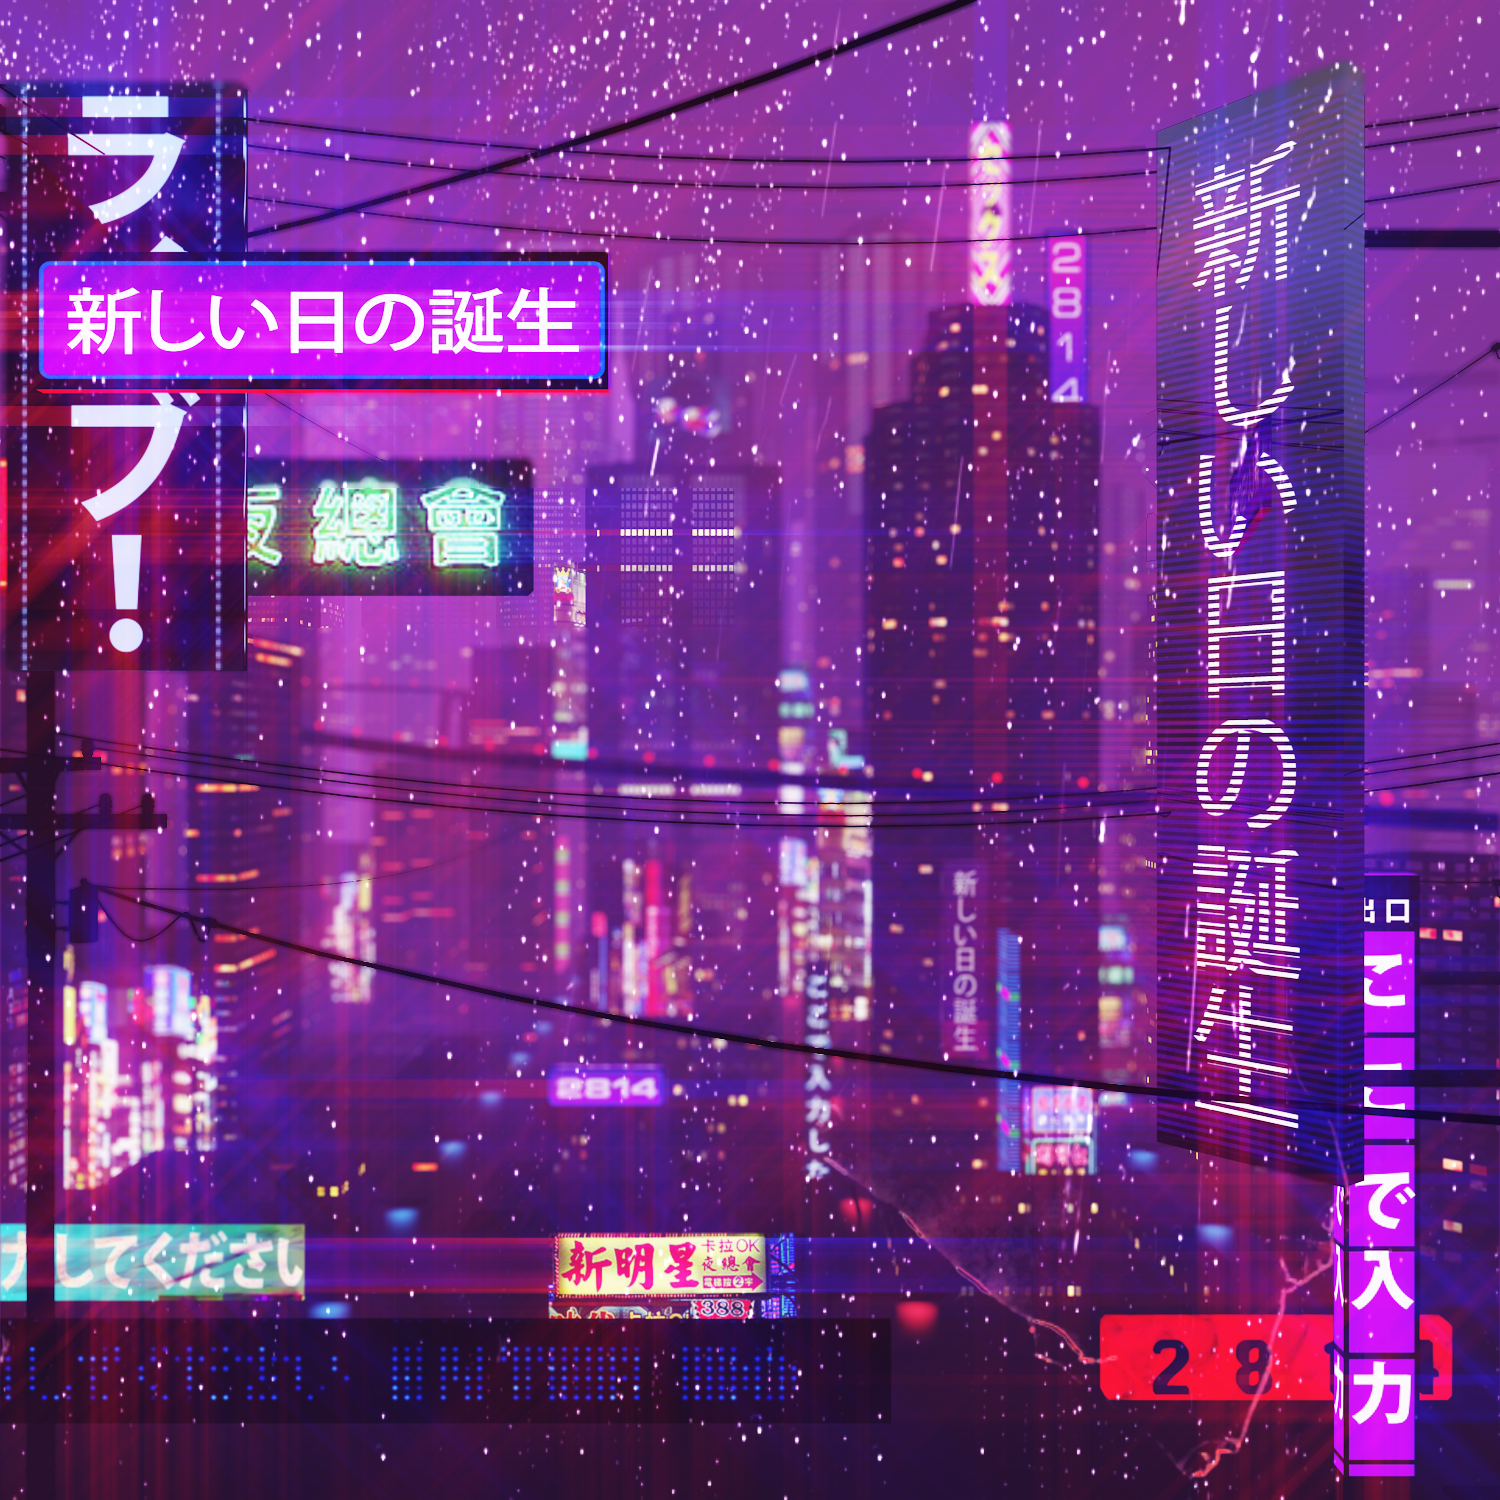
\includegraphics[width=0.2\textwidth]{../data/test-image.png}
  \end{subfigure}%
  \begin{subfigure}
    \centering
    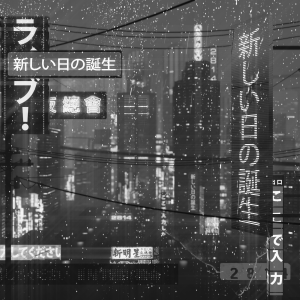
\includegraphics[width=0.2\textwidth]{../data/image-original.png}
  \end{subfigure}
  \begin{subfigure}
    \centering
    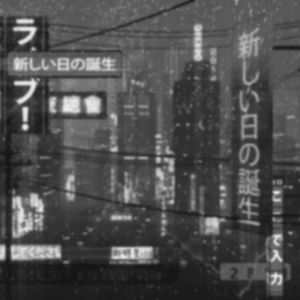
\includegraphics[width=0.2\textwidth]{../data/image-blurred.png}
  \end{subfigure}
\end{figure}
\end{itemize}
\end{itemize}
\end{itemize}
\end{itemize}
\end{enumerate}
\item Repa Representation
\label{sec-2-2}
\begin{itemize}
\item This representation comes from the fact that I wanted the code to
run on the full 1500x1500 version of the images above, and I spent
hours trying to debug why \texttt{Word16} slowed down the program so much.
\item Repa also gives me tools to do this work rather easily, so I'll
break this section into 3 parts
\begin{enumerate}
\item What is REPA and why did it take me to understand what Ι was doing
\item Working just on Grey images
\item Working on both grey and colored images
\end{enumerate}
\end{itemize}
\begin{enumerate}
\item What is REPA and why did it take me to understand what Ι was doing
\label{sec-2-2-1}
\begin{itemize}
\item so REPA is a library for high performance regular multi-dimensional
parallel arrays.
\item This means a few things
\begin{enumerate}
\item we don't have to say a word about parallelism and our code will
still be run in parallel (I ended up getting 100\% on all 8 of my cores!)
\item REPΑ is rather fast and memory efficient
\item REPA due to its "multi-dimensional" nature has rather complex
type signatures and makes grokking it rather hard at first
\end{enumerate}
\item So REPA achieves its speed in a rather interesting way, whenever
a function is invoked, REPA doesn't actually make an array
\begin{verbatim}
a = fromListUnboxed (Z :. 4 :. 4) [1..16] :: Array U DIM2 Int
R.map (+ 1) a :: Array D DIM2 Int
\end{verbatim}
\begin{itemize}
\item so here we make an unboxed array (that's what U means) of dimension 4 by 4 (that's what
Z :. \ldots{} means) with type Int inside.
\item when we run map over the entire array instead of getting another
Unboxed type U back, we instead get the type \texttt{Array D DIM2 Int}
back, where D means that this array is really just functions from
indices to elements. So the array never really exists in memory
\item this is rather useful, as this map can be fused out and the
intermediate arrays never exist
\end{itemize}
\item Another note is the shape, the (Z :. 4 :. 4) notation denotes the
shape of the array, and this data structure is best to be thought of
as a reverse list
\item even with understanding both of these points, it took me more than
just a few hours to fully understand how to use the library, and in
the following two sections I'll try to explain the logic of what is happening.
\end{itemize}
\item Working just on Grey images
\label{sec-2-2-2}
\begin{itemize}
\item so like the matrix representation Ι decided to once again only work
on grey images at first
\item the code for both these sections are in RepaHelper.hs
\item The first step was trying to figure out how to turn an Image into a
Repa array.
\begin{verbatim}
-- only going to be working on 2D images for now, trying to figure out slices is too much
imageToGreyRepa :: LumaPlaneExtractable a ⇒ Image a → Array D DIM2 (PixelBaseComponent a)
imageToGreyRepa img@(Image w h _) = R.fromFunction (Z :. w :. h) f
  where f (Z :. i :. j) = pixelAt newImg i j
        newImg          = extractLumaPlane img
\end{verbatim}
\begin{itemize}
\item so I end up representing a grey image as a 2D array (DIM2 stands
for dimension 2).
\item I do this by making a function that takes an image (an image
consists of the width, height, and data) which we call img with
width w and height h, and returning our array
\item this array never really gets materialized, as we just make the
array from a function that just queries the greyed version of the image
\end{itemize}
\item Now that we have the image in the data that we can work with, we
must now make our Gaussian once again
\begin{verbatim}
gausianStencilX :: Num a ⇒ Stencil DIM2 a
gausianStencilY :: Num a ⇒ Stencil DIM2 a
gausianStencilX = [stencil2| 1 4 6 4 1 |]
gausianStencilY = [stencil2| 1
                             4
                             6
                             4
                             1 |]
\end{verbatim}
\begin{itemize}
\item this code is a bit special. So Repa has a stencil library that was
made to basically apply any arbitrary kernel as long as it's
smaller than 7x7
\item so these two represent the Gaussian and give other data to our
function below
\end{itemize}
\begin{verbatim}
blurGausX :: (Source r b, Fractional b) ⇒ Array r DIM2 b → Array D DIM2 b
blurGausY :: (Source r b, Fractional b) ⇒ Array r DIM2 b → Array D DIM2 b
blurGausX = R.map (/ 16) . mapStencil2 BoundClamp gausianStencilX
blurGausY = R.map (/ 16) . mapStencil2 BoundClamp gausianStencilY

blur :: (Source r b, Fractional b) ⇒ Array r DIM2 b → Array D DIM2 b
blur = blurGausX . blurGausY
\end{verbatim}
\begin{itemize}
\item The library is kind enough to give us a mapStencil over a 2D
array, so really we just map the Gaussian and then divide by 16, and compose
both of them to get the blur

\item The stencil probably runs in parallel, though I'm not quite sure
where the parallelization is coming from (might be even before
this point!)
\end{itemize}

\item So now that we have the blur filter working, we just have to make a
conversion function then run it
\begin{verbatim}
repaToGreyImage :: (RealFrac a, Source r a) ⇒ Array r DIM2 a → Image Word8
repaToGreyImage xs = generateImage create width height
  where Z :. width :. height = R.extent xs
        create i j           = round (xs ! (Z :. i :. j)) :: Word8
\end{verbatim}
\begin{itemize}
\item once again we use generateImage and grab the proper coordinates
\end{itemize}

\item So now lets run the image blur again but on a bigger version of the
same image!
\begin{verbatim}
mainRepaGrey = do
  x <- testImage
  let y = R.imageToGreyRepa x
  let z = R.blur $ R.map fromIntegral y
  savePngImage "./repa-test-real.png" (ImageY8 (R.repaToGreyImage z))
\end{verbatim}
\begin{itemize}
\item this code basically grabs the image and runs our functions
\item and once again we save the pngs which can be viewed below
\item I've had to scale the image down for the PDF, so do use my
directories and look at "repa-big-test" and "test-big"
\item So the image on the left below is the original
\item And the image on the right is the blurred version
\begin{figure}
  \centering
  \begin{subfigure}
    \centering
    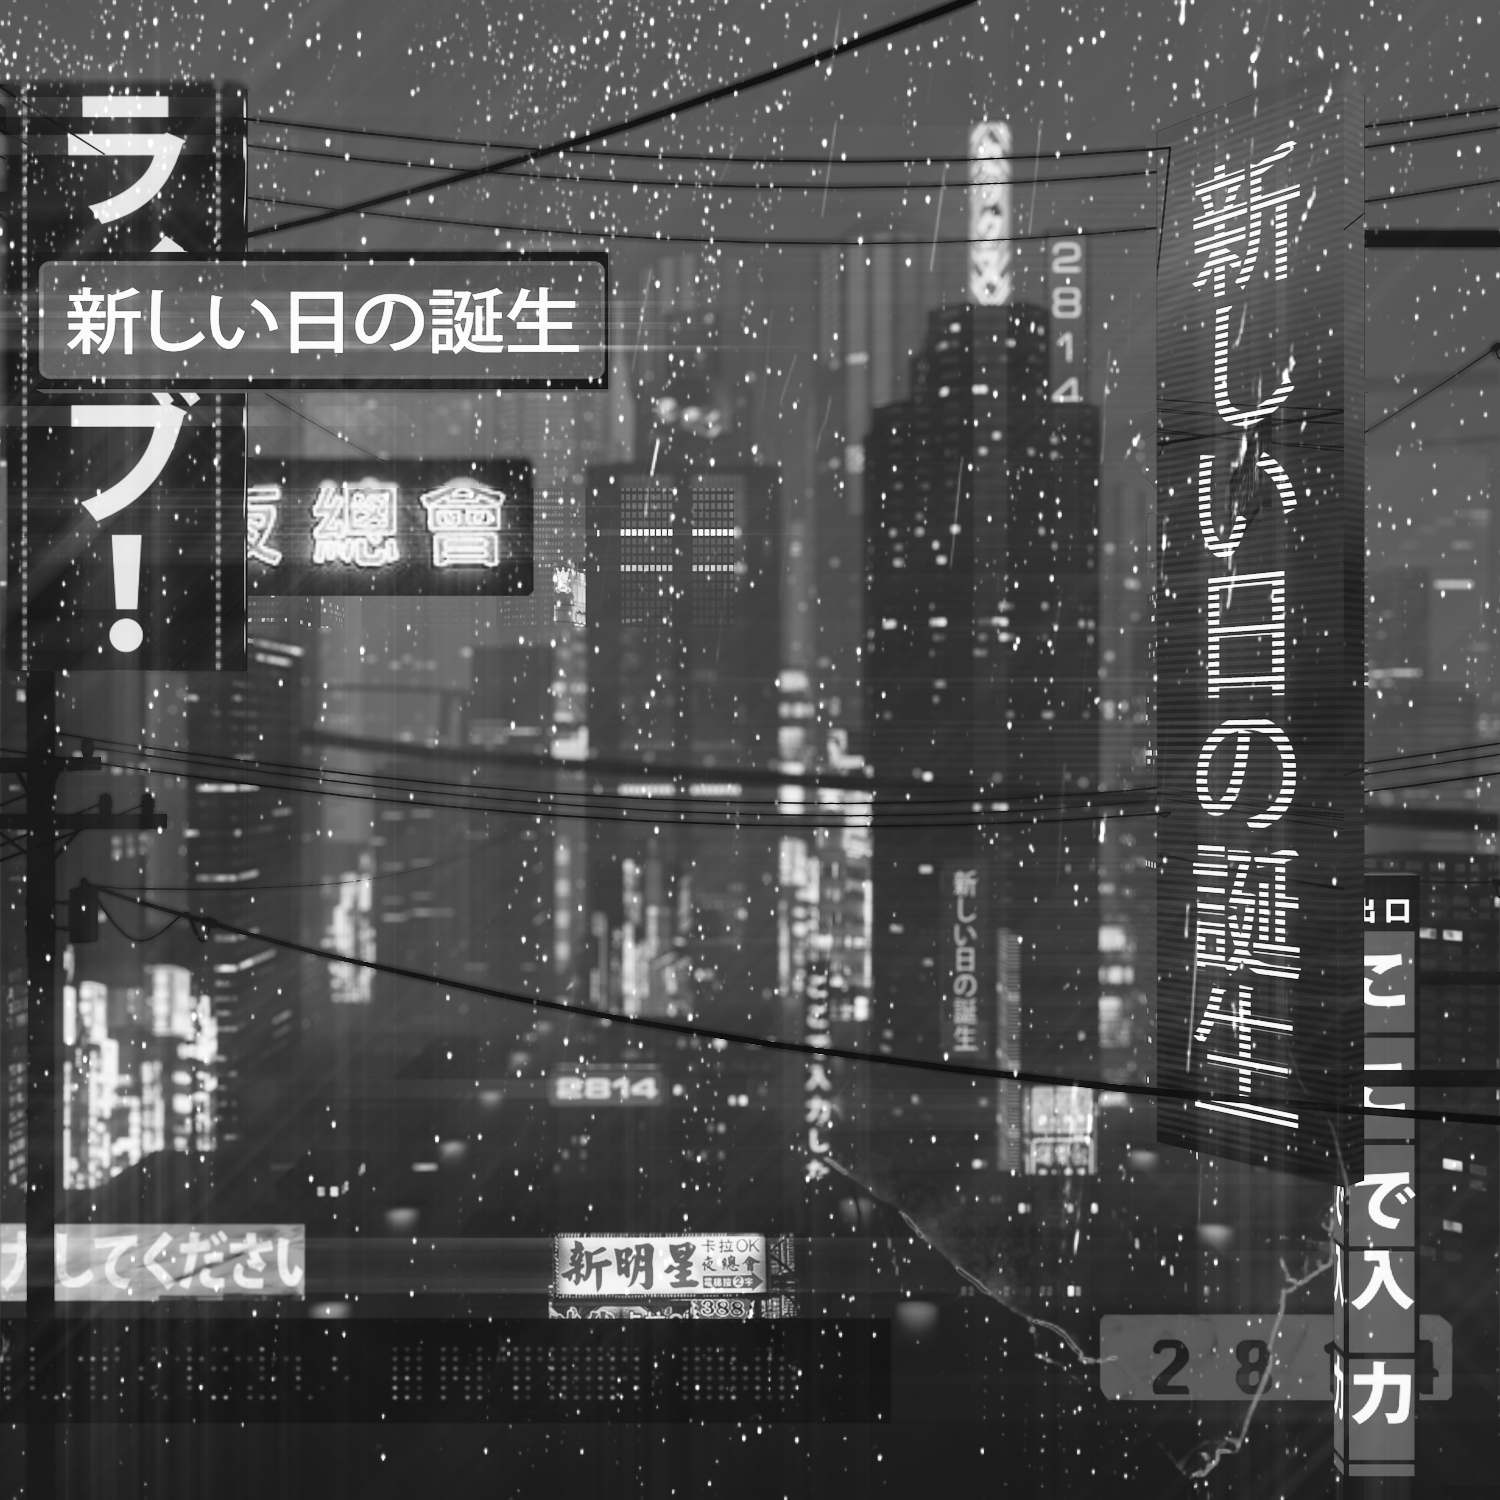
\includegraphics[width=0.4\textwidth]{../data/test-big.png}
  \end{subfigure}%
  \begin{subfigure}
    \centering
    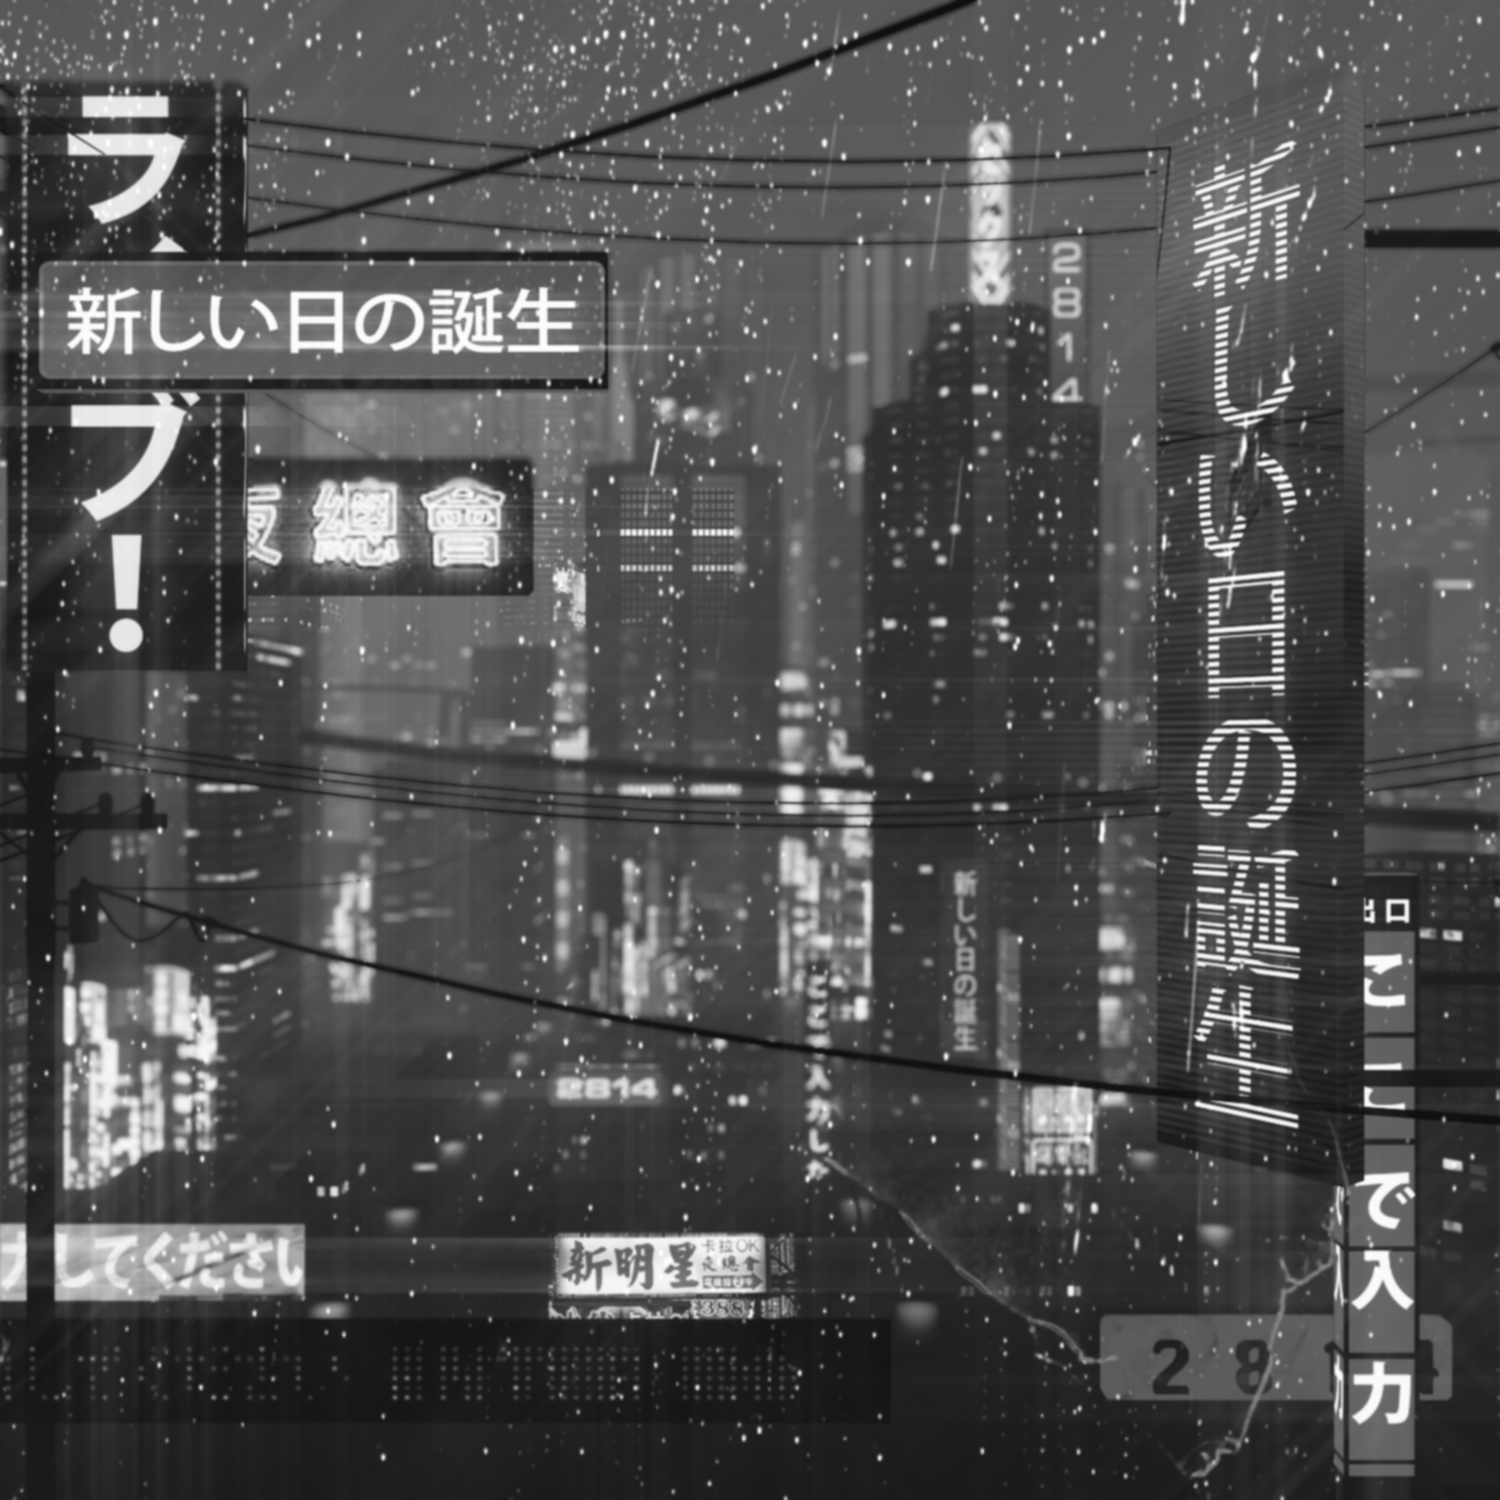
\includegraphics[width=0.4\textwidth]{../data/repa-big-test.png}
  \end{subfigure}
\end{figure}
\item I ended up scaling the images to .4, as the blurring is more
subtle on bigger image
\item 
\end{itemize}
\end{itemize}
\item Working on both grey and colored images
\label{sec-2-2-3}
\begin{itemize}
\item this section in particular took a lot of effort as it took me quite
a while to grok how slices work in this library and how to properly
use the tools
\item Reading an image to a REPA array is already done for me as there is
a \texttt{readImageRGB} function provided in JuicyPixels-repa, so I don't
have to worry about that part
\item to get a grip on the tools, I thought Ι would make
repaExtractWindows which really isn't used
\begin{verbatim}
repaExtractWindows :: (Source r a) => Int -> Int -> Array r DIM3 a -> Array D DIM3 (Array D DIM3 a)
repaExtractWindows row col arr = R.fromFunction (Z :. i - row :. j - col :. k) grabsubs
  where Z :. i :. j :. k = R.extent arr
        grabsubs sh      = R.extract sh (Z :. row :. col :. 1) arr
\end{verbatim}
\begin{itemize}
\item I made this as I was confused on how to get subsection of the
array properly. At first \texttt{R.fromFunction} used to be \texttt{R.traverse}
that took an array and did some calculations, but it turned out to not
be needed
\item there is a nifty function called extract which I can give it a
shape of where to start and how big it is.
\end{itemize}
\item Now that Ιwas understanding what I was doing, we can now make
blurCol
\begin{verbatim}
data MyImage a = RGB a a a | RGBA a a a a | Grey a

fromList :: [a] -> MyImage a
fromList [a,b,c]   = RGB a b c
fromList [a,b,c,d] = RGBA a b c d
fromList [a]       = Grey a
fromList _         = error "not a valid image"

blurCol :: (Fractional e, Source r e) => Array r DIM3 e -> Array D DIM3 e
blurCol = flip reshape . f . fromList . fmap blur . slices <*> R.extent
  where f (RGBA a b c d) = interleave4 a b c d
        f (RGB a b c)    = interleave3 a b c
        f (Grey a)       = a

slices :: Source r e => Array r DIM3 e -> [Array D DIM2 e]
slices arr = f <$> [0..(k-1)]
  where
    (Z :. _ :. _ :. k) = R.extent arr
    f a                = slice arr (Z :. All :. All :. (a :: Int))
\end{verbatim}
\begin{itemize}
\item I broke this function up into 3 discrete pieces, my custom data
type, blurCol, and slices

\begin{itemize}
\item \uline{Slices}
\begin{itemize}
\item slices takes an array and stuffs the 3rd dimension of the array
into its own list while keeping all x and y coordinates of the array
\item this leaves us with a list of 2D arrays, which means the old
blur filter can work
\end{itemize}
\item \uline{MyImage}
\begin{itemize}
\item this data type was mostly a response to the interleave
functions. due to how strict Haskell is with its types Ι can't
just check the size of the list I get from slices and decide on
which one I want
\item so I created this data type just to facilitate the interleave
functionality
\begin{itemize}
\item interleave just interleaves all elements in the arrays given
to it
\end{itemize}
\item Also note at first I used R.++ instead, but that ended up
splitting they image into 3 versions of the original image
\end{itemize}
\item \uline{blurCol}
\begin{itemize}
\item blurCol is where the magic happens, now that we have 2D
slices, we can now just call blur on each slice and combine it
with interleave. Finally we get a 2D array back, so we just
reshape the array into a 3rd dimensional one
\end{itemize}
\end{itemize}
\end{itemize}

\item All that is left is converting the array into a 3D one. there is
actually a function called \texttt{imgToImage :: Img a → DynamicImage} but
oddly enough it segfaults (it uses some weird foreign pointer
magic), so I made my own once again
\begin{verbatim}
repaToRGBImage :: (RealFrac a, Source r a) ⇒ Array r DIM3 a → Image PixelRGB8
repaToRGBImage arr = generateImage create height width -- may have mixed up the width and height at some point
  where
    Z :. width :. height :. _ = R.extent arr
    create i j                = PixelRGB8 (grab 0) (grab 1) (grab 2)
      where grab k = round $ arr ! (Z :. j :. i :. k) :: Word8
\end{verbatim}

\begin{itemize}
\item So this code looks a lot like the grey image converter, however
there is one weird difference, and that is in the generate image I
give it height then width, and Ι index my array with j then i
instead of i then j. I think something might have been flipped at
once point, I'm not too sure, but this works like a charm.

\item A previous version used to use foldl1 with the PixelRGB8 and keeping
the computation in the list, but since Ιused the wrong fold, I
ended up mixing up R and B on the final image which I will show with
the rest.
\end{itemize}

\item So now lets run and see what we get!
\begin{verbatim}
main = do
  x <- C.readImageRGB "./data/Color-test.png"
  let y = case x of Left _ -> error "image not found"; Right z -> z
  let z = R.blurCol (R.map fromIntegral (imgData y))
  z' <- R.computeUnboxedP z :: IO(R.Array R.U R.DIM3 Double)
  let z'' = R.repaToRGBImage z'
  savePngImage "./Color-save.png" (ImageRGB8 z'')
\end{verbatim}
\begin{itemize}
\item the computeUnboxedP is the only parallel code I've written, which
just tells the array to be computed in parallel, idk if this
speeds up the computation however.
\item but lets see the fruits of our labor. I would suggest looking in
the data director and look at "Color-test"
"Color-save-proper-colors" and "Color-save-proper-colors" for the
full size images
\item the left is the original
\item the right was the mistaken R B flip and blurred
\item and the bottom is the blurred version of the first
\begin{figure}
  \centering
  \begin{subfigure}
    \centering
    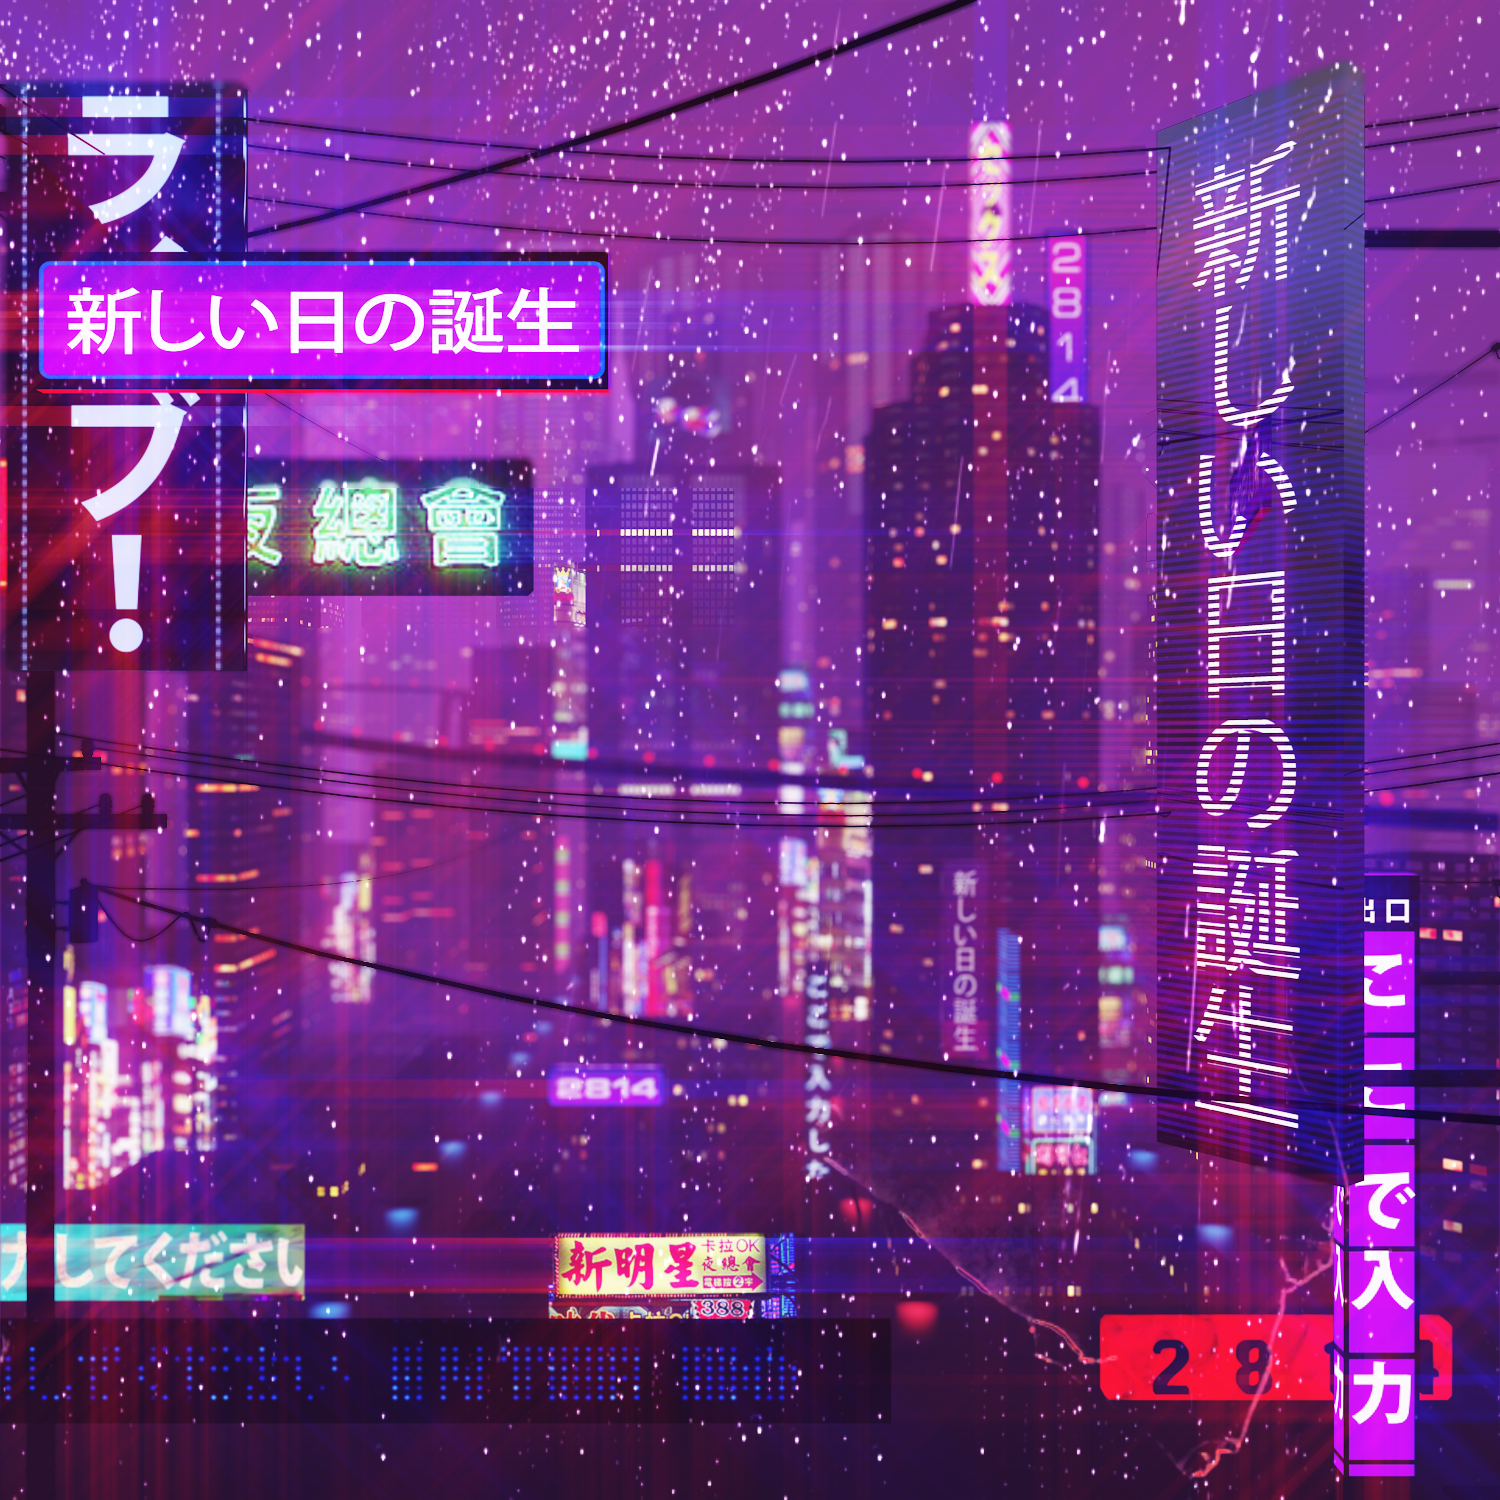
\includegraphics[width=0.4\textwidth]{../data/Color-test.png}
  \end{subfigure}%
  \begin{subfigure}
    \centering
    \includegraphics[width=0.4\textwidth]{../data/Color-save-inverted-red-blue.png}
  \end{subfigure}
  \begin{subfigure}
    \centering
    \includegraphics[width=0.4\textwidth]{../data/Color-save-proper-colors.png}
  \end{subfigure}
\end{figure}
\end{itemize}
\item 
\end{itemize}
\item Overall
\label{sec-2-2-4}
\begin{itemize}
\item this approach was rather fast clocking in at less than 15 seconds
real time and not taking up more than 89 MB of memory while working all
my cores to 100\%
\end{itemize}
\end{enumerate}
\end{enumerate}
% Emacs 25.3.1 (Org mode 8.2.10)
\end{document}